
En este capítulo se presentan los detalles de diseño del proyecto, basándonos en el
análisis mostrado en los anteriores apartados. Se detallan la arquitectura general
y el diseño físico de datos entre otros aspectos.

%%%%%%%%%%%%%%%%%%%%%%%%%%%%%%%%%%%%%%%%%%%%%%%%%%%%%%
%%%%%%%%%%%%%%%%%%%%%%%%%%%%%%%%%%%%%%%%%%%%%%%%%%%%%%

\section{Arquitectura del sistema}

\subsection{Arquitectura física}

En este apartado, describimos los principales componentes hardware que forman
la arquitectura física de nuestro sistema.

\paragraph{Hardware}
El hardware mínimo indispensable para la correcta ejecución del motor del
proyecto se detalla en la siguiente lista:

\begin{itemize}
    \item 512MiB de memoria RAM como mínimo.
    \item 10GiB de disco duro como mínimo.
\end{itemize}

\paragraph{Software}

En cuanto al software necesario para la ejecución del proyecto, se detallan los
siguientes elementos, que es necesario instalar para desplegar el sistema:

\begin{itemize}
    \item Sistema operativo \textbf{GNU/Linux}, preferiblemente basado en paquetería Debian.
    \item Código fuente del proyecto \textbf{Sitic}.
    \item Intérprete de \textbf{Python}, versión mínima 2.7.
    \item Soporte de entornos virtuales \textbf{VirtualEnv} para la encapsulación de dependencias.
\end{itemize}

\subsection{Arquitectura lógica}

La arquitectura lógica del sistema está formada por los elementos software
(servicios, aplicaciones, librerías, frameworks, etc.) que componen el software base,
más el software desarrollado para cumplir los requisitos de la aplicación. En esta
sección se muestra la organización de los distintos elementos software que
componen el proyecto así como la comunicación entre ellos.

En la figura~\ref{fig:arquitectura-logica}  se puede ver un esquema de cómo se comunican los diferentes
elementos que conforma el sistema a alto nivel. En detalle, el flujo que sigue
en cada capa es el siguiente:

\begin{figure}[htbp]
    \centering
    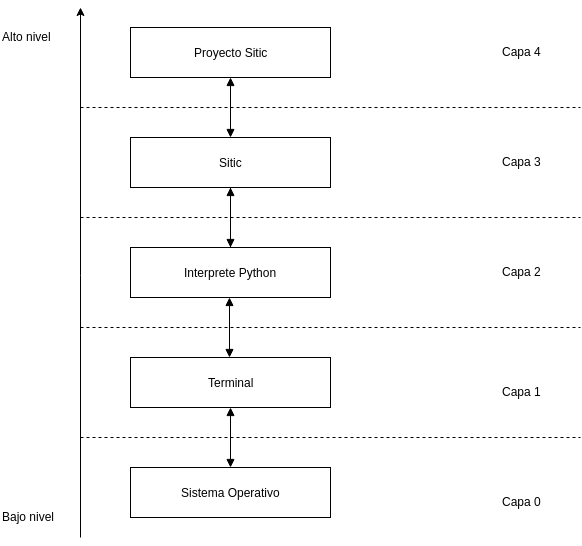
\includegraphics[width=0.9\textwidth]{5_diseno/arquitectura_logica}
    \caption{Arquitectura lógica}
    \label{fig:arquitectura-logica}
\end{figure}

De esta forma, en este apartado de arquitectura lógica, vamos a describir todos los elementos
software que componen el software base de la aplicación, además del propio software a desarrollar.
De esta forma, podemos citar los siguientes componentes software:

\begin{itemize}
    \item Primeramente, como acabamos de comentar, nos encontramos el elemento software que
        compone a nuestro proyecto, como ya se ha descrito anteriormente, un generador de sitios web estáticos.
    \item Esta herrameinta está desarrollado haciendo uso del lenguaje de programación Python, por lo que es
        indispensable que la máquina donde se use la herramienta, tenga el lenguaje disponible.
    \item A su vez, dicho proyecto se ejecutará usando una terminal. La terminal del sistema debe de
        tener como requisito poder ejecutar código Python.
    \item Por último, el sistema operativo donde se vaya a instalar todos los componentes anteriores,
        debe de tener soporte tanto para el servidor web donde vamos a incluir nuestro proyecto,
        como para la tecnología Python, ya que el resto de componentes comentados, funcionan
        sobre estas dos piezas. Por suerte, Python es un lenguaje de programación multiplataforma,
        el cual tiene soporte para los principales sistemas operativos existentes en la actualidad.
\end{itemize}

%%%%%%%%%%%%%%%%%%%%%%%%%%%%%%%%%%%%%%%%%%%%%%%%%%%%%%
%%%%%%%%%%%%%%%%%%%%%%%%%%%%%%%%%%%%%%%%%%%%%%%%%%%%%%

\section{Diseño detallado de componentes}

En esta sección se detalla el diseño concreto de algunos componentes de la aplicación,
especificando las clases involucradas y el flujo de mensajes entre ellas.

En particular, se han elegido el proceso parseo y generación de contenidos
por ser el que mayor importancia y complejidad tiene.

\subsubsection{Parseo y generación de contenidos}

El proceso de parseo y generación de contenidos es un proceso que involucra bastantes
elementos y es el componente esencial de la herramienta.

\begin{figure}[htbp]
    \centering
    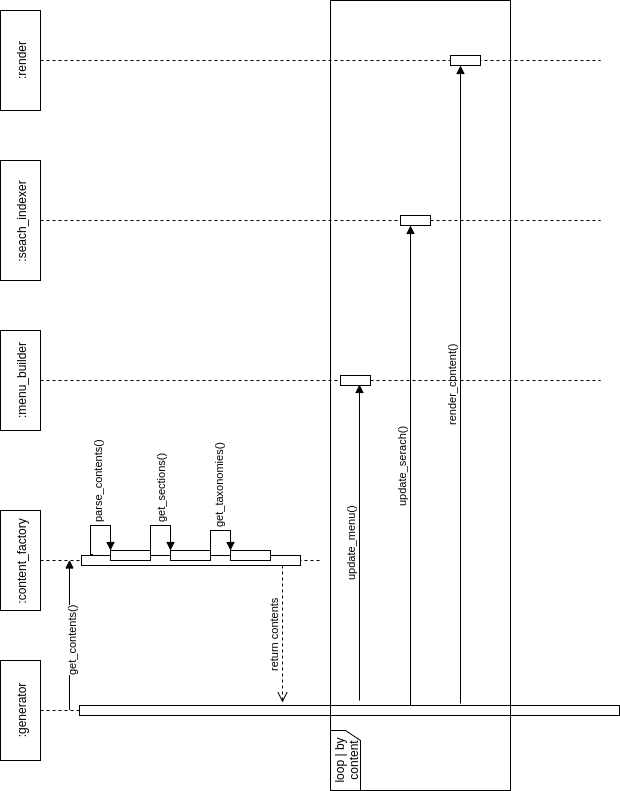
\includegraphics[width=1.1\textwidth]{5_diseno/diagrama_secuencia}
    \caption{Diagrama de secuencia}
    \label{fig:diagrama_secuencia}
\end{figure}

En primer lugar, cuando el usuario ejecuta la generación de contenidos, ejecutando el comando
principal de la herramienta, el sistema recorre todos y cada uno de los ficheros que se encuentran
en la carpeta de contenidos definida.

Cada fichero lo separa en dos partes, la parte que contiene los metadatos del contenido y la parte que
contiene el contenido redactado. Una vez hecho esto parsea cada una de las partes para convertirlos en
un tipo de datos que sea de fácil manipulación, los metadatos los convierte a un tipo de datos
diccionario del lenguaje Python y el contenido en sí, lo parsea en función de la extensión que se le
haya puesto al fichero, que determinará que lenguaje de marcado hemos utilizado.

Una vez que todos los ficheros han sido parseados, determinar qué ficheros se van a generar, ya que
el usuario puede haber definido en los metadatos de estos que el fichero haya caducado o que simplemente
no esté listo para ser publicado aún y esté marcado como borrador.

Teniendo ya los ficheros que se van a publicar, se recopilan el resto de contenidos a partir de estos, es decir,
todos aquellos contenidos que depende de estos como son la homepage, las secciones o las taxonomías,
ya que si, por ejemplo, existe una sección con un único contenido, se evita que dicha sección se genere
completamente vacía.

Tras esto, se recorre cada uno de los ficheros, determinando que template se debe usar como base para renderizarlos,
y se le comunica al motor de templates Jinja, el contenido que debe de renderizar en la template.

Por último, el sistema mueve todos los ficheros estáticos(CSS, imágenes, Javascript) que la web pueda necesitar
a la carpeta con todos los contenidos generados.


%%%%%%%%%%%%%%%%%%%%%%%%%%%%%%%%%%%%%%%%%%%%%%%%%%%%%%
%%%%%%%%%%%%%%%%%%%%%%%%%%%%%%%%%%%%%%%%%%%%%%%%%%%%%%

\section{Diagrama de clases de diseño}

A continuación se muestra el diagrama de clases de diseño. Que se ha tenido que dividir en dos partes
para su correcto visionado.

\begin{figure}[htbp]
    \centering
    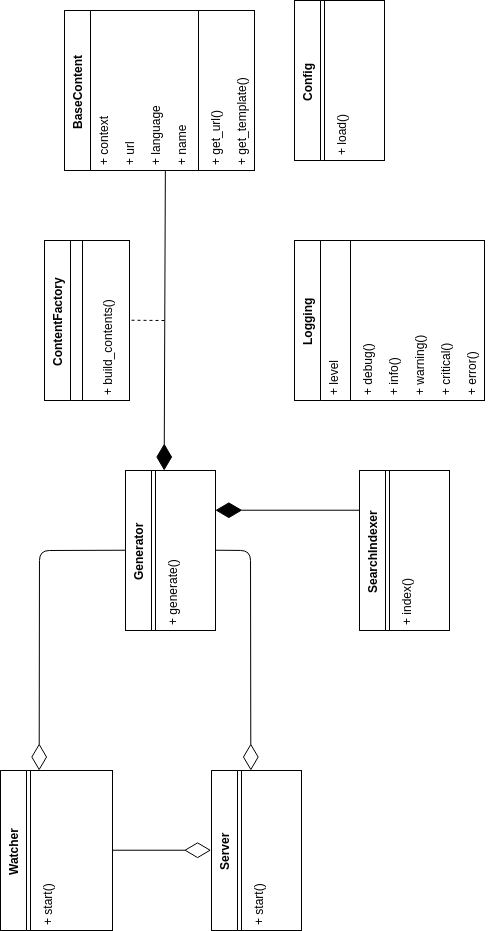
\includegraphics[width=0.8\textwidth]{5_diseno/clases_de_diseno1}
    \caption{Diagrama de clases de diseño 1}
    \label{fig:clases_diseno}
\end{figure}

\begin{figure}[htbp]
    \centering
    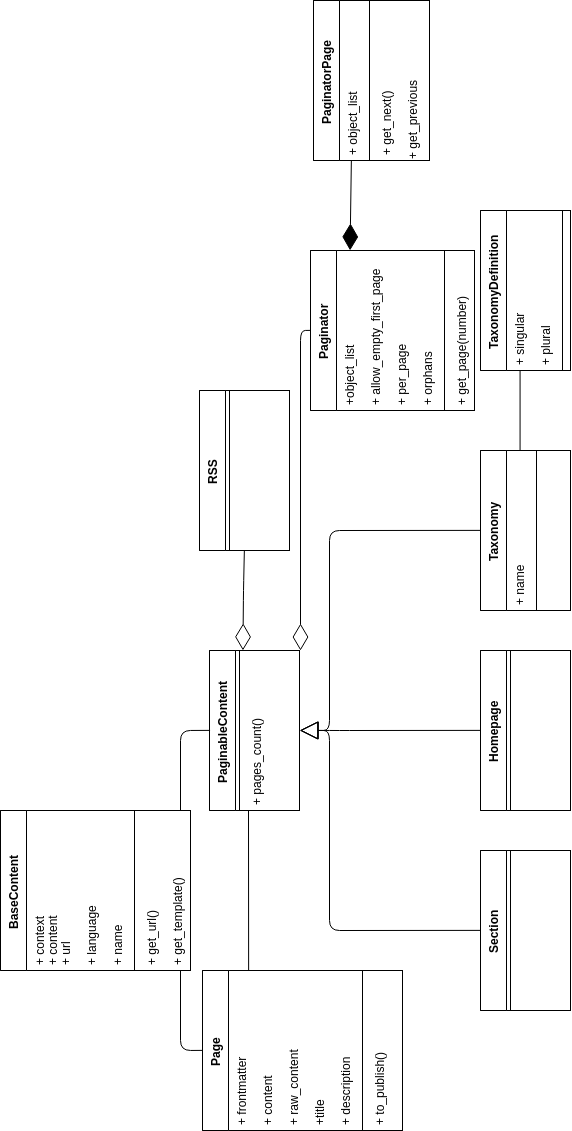
\includegraphics[width=0.8\textwidth]{5_diseno/clases_de_diseno2}
    \caption{Diagrama de clases de diseño 2}
    \label{fig:clases_diseno}
\end{figure}

En el diagrama de clases de pueden apreciar clases que no están relacionadas
con ninguna otra del diagrama. Estas clases a las que nos referimos siguen un patrón Singleton~\cite{singleton}, que
permite que cualquier clases pueda acceder a ella desde cualquier parte del sistema. Sólo existirá una
única instancia de cada una de las clases Singleton, que se creará en la primera llamada que se realice a
ellas.

%%%%%%%%%%%%%%%%%%%%%%%%%%%%%%%%%%%%%%%%%%%%%%%%%%%%%%
%%%%%%%%%%%%%%%%%%%%%%%%%%%%%%%%%%%%%%%%%%%%%%%%%%%%%%

% \section{Diseño de interfaz de usuario}
